\section{Backen}\label{sec:backen}
\textbf{Hinweis}: In diesem Kapitel sind Rezepte, die ein wenig fortgeschritten sind.
Es erfordert ein gefühl für Teig, im besonderen Hefeteige, um die Rezepte wirklich umsetzen zu können.
Zeiten, wie sie in den Rezepten aufgeführt sind, sind nur grobe Anhaltspunkte, die abhängig von der Temperatur, mit der die Teige geführt werden um Faktoren anders sein können.
\newpage
\subsection{Münchner Brezen oder Brezensemmeln}\label{subsec:brezen-oder-brezensemmeln}
\begin{tcolorbox}
    [
    blanker,
    width=0.64\textwidth,enlarge left by=0.36\textwidth,
    before skip=6pt,
    breakable,
    overlay unbroken and first={%
        \node[inner sep=0pt,outer sep=0pt,text width=0.33\textwidth,
            align=none,
            below right]
        at ([xshift=-0.36\textwidth]frame.north west)
            {%% left
            Rezept von Jakob\\
            Rezept für 10 Brezen\\
            \begin{flushright}
                \noindent\makebox[\linewidth]{\rule{\linewidth}{0.4pt}}
                \textbf{Vorteig}\\
                80g Weizenmehl, Type 550\\
                80g Wasser, Zimmerwarm\\
                0,1g Hefe\\
                \textbf{Mehlkochstück}\\
                260g Wasser\\
                50g Weizenmehl, Type 550\\
                11g Salz\\
                \textbf{Hauptteig}\\
                Vorteig\\
                Mehlkochstück\\
                21g Wasser\\
                10g Frischhefe\\
                13g Butter oder Alsan\\
                475g Weizenmehl, Type 550\\
            \end{flushright}
        };}]
%% right
    \begin{figure}[H]
        \begin{center}
            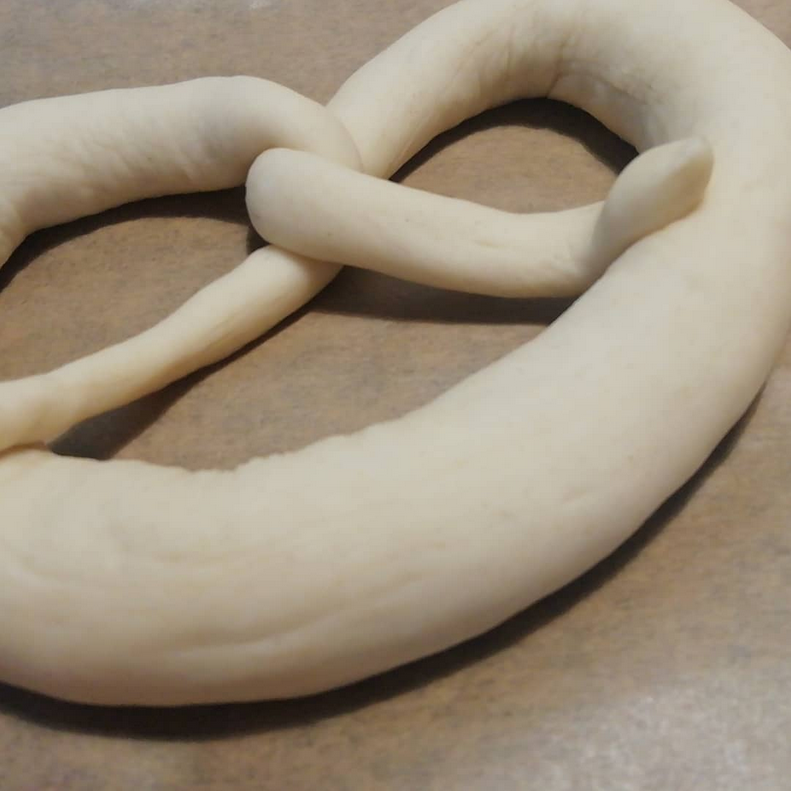
\includegraphics[width=0.75\linewidth]{img/breze}
            \caption{Geschlungene Breze vor dem Backen}
        \end{center}
    \end{figure}
%%%%%%%%%% Rezept Anleitung %%%%%%
    \textbf{Hinweis}: In diesem Kapitel sind Rezepte, die ein wenig fortgeschritten sind.
    Es erfordert ein gefühl für Teig, im besonderen Hefeteige, um die Rezepte wirklich umsetzen zu können.
    Zeiten, wie sie in den Rezepten aufgeführt sind, sind nur grobe Anhaltspunkte, die abhängig von der Temperatur, mit der die Teige geführt werden um Faktoren anders sein können.\\

    Alle Vorteigzutaten vermischen und 20 Stunden bei Zimmertemperatur (ungefähr $20^\circ C$) reifen lassen.\\

    Für das Mehlkochstück alle Zutaten unter ständigem Rühren aufkochen lassen.
    Nach etwas abkühlen das Mehlkochstück mit Frischhaltefolie auf der Oberfläche abdecken, um Hautbildung zu verhindern.
    Anschließend für mindestens 4 Stunden, besser aber mindestens 12 Stunden quellen lassen.\\

    Für den Hauptteig sämtliche Zutaten 5 Minuten auf der niedrigsten Stufe kneten lassen (Küchenmaschine).
    Dann weitere 8 Minuten auf einer mittleren Einstellung kneten.
    Der Teig sollte fest, straff und nicht klebrig sein.\\
    60 Minute Gare bei $20^\circ C$.
    Alle 30 Minuten den Teig ausstoßen.\\
    Teiglinge zu 90g abstechen und rundschleifen.
    Teiglinge 10 Minuten ruhen lassen.
    Für Brezensemmeln die folgenden Schritte ignorieren, aber die Garzeiten trotzdem weiter befolgen.
    Die Teiglinge zu circa 40cm langen Strängen rollen und anschließend nochmals 5-10 Minuten ruhen lassen.
    Stränge auf 50-60cm Länge dehnen/rollen und die Brezen schlingen.
    Brezen auf nahezu vollreife reifen lassen.
    Brezen auf Backpapier setzen und 15 Minuten möglichst Kühl absteifen lassen.\\
    In 4\%iger Natronlauge 4 Sekunden laugen und anschließend mit Salz bestreuen.\\
    Bei $230^\circ C$ ohne Dampf backen.
    Die Ofentür möglichst einen Spalt öffnen, um eine trockene Backatmosphäre zu schaffen.
\end{tcolorbox}
\newpage

\subsection{Focaccia}
\begin{tcolorbox}
    [
    blanker,
    width=0.64\textwidth,enlarge left by=0.36\textwidth,
    before skip=6pt,
    breakable,
    overlay unbroken and first={%
        \node[inner sep=0pt,outer sep=0pt,text width=0.33\textwidth,
            align=none,
            below right]
        at ([xshift=-0.36\textwidth]frame.north west)
            {%% left
            Rezept von Jakob\\
            Rezept für 1 Focaccia\\
            \begin{flushright}
                \noindent\makebox[\linewidth]{\rule{\linewidth}{0.4pt}}
                \textbf{Vorteig}\\
                190g Weizenmehl, Type 550\\
                190g Wasser, Zimmerwarm\\
                0,2g Hefe\\
                \textbf{Hauptteig}\\
                Vorteig\\
                360g Weizenmehl, Type 550\\
                238g Wasser\\
                4g Frischhefe\\
                10g Salz\\
                \textbf{Belag}\\
                Nach Belieben
                Menge Zutat
            \end{flushright}
        };}]
%% right
    \begin{figure}[H]
        \begin{center}
            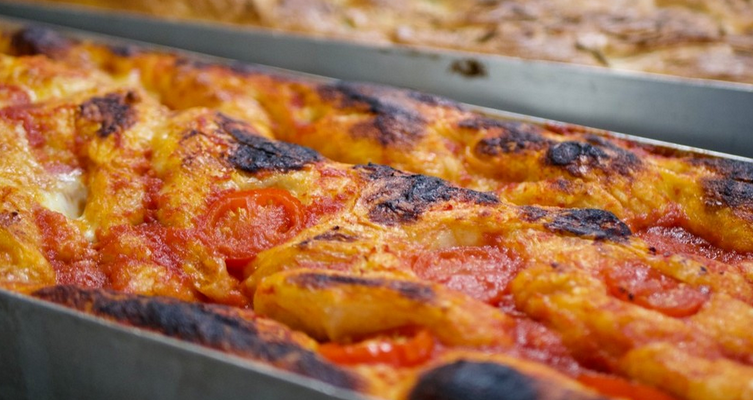
\includegraphics[width=\linewidth]{img/focaccia}
            \caption{Bild}
        \end{center}
    \end{figure}
%%%%%%%%%% Rezept Anleitung %%%%%%
    \textbf{Hinweis}: In diesem Kapitel sind Rezepte, die ein wenig fortgeschritten sind.
    Es erfordert ein gefühl für Teig, im besonderen Hefeteige, um die Rezepte wirklich umsetzen zu können.
    Zeiten, wie sie in den Rezepten aufgeführt sind, sind nur grobe Anhaltspunkte, die abhängig von der Temperatur mit der die Teige geführt werden um Faktoren anders sein können.\\

    Die Vorteigzutaten vermischen und 14-18 Stunden bei Zimmertemperatur ($20^\circ C$) reifen lassen.\\
    Hauptteigzutaten vermischen und dann 7 Minuten auf der niedrigsten Stufe kneten lassen (Küchenmaschine).
    Dann weitere 5 Minute auf einer mittleren Stufe kneten lassen.\\
    Den Teig 2,5 Stunden gehen lassen.
    Dabei alle 30 Minuten dehnen und falten.\\
    Den Teig auf ein kräftig mit Olivenöl bestrichenes Blech geben.
    Mit den Fingern den Teig versuchen so gut wie möglich auf dem Blech verteilen.
    10 Minuten abgedeckt ruhen lassen.
    Danach wieder mit den Fingern den Teig nochmals auf dem Blech verteilen.
    Weitere 10 Minuten abgedeckt ruhen lassen.\\
    Jetzt den Belag auf dem Teig verteilen.
    Weitere 30 Minuten ruhen lassen.
    Dann können die typischen  \glqq Löcher \grqq{} mit den Fingern in den Teig gestochen werden.\\
    Die Focaccia bei $250^\circ C$ 20 Minuten backen.
\end{tcolorbox}
\newpage
